Designovervejelser
Vi har valget at lave et program der planlægger skema for udskolingssektoren på en givende skole. Vi har valgt det skal være udskoling, altså 7, 8 og 9 klasse, for at kunne simulerede at lærerne kan have klasser på tværs af klassetrinene, og der ved vise at software løsningen kan løse problemet med sammenhængene forberedelsestimer for lærerne. Derudover skal programmet kunne planlægge skemaerne således at det er muligt at have samarbejde på tværs af parallel klasserne\cite{interview}.  Da det er udskoling der arbejdes videre med, skal der specificeres hvilke parametre der gælder for disse klassetrin. Alle klassetrinene skal undervises i dansk, idræt, matematik, engelsk, historie, biologi, geografi, fysik og kemi, tysk eller fransk, derudover skal de have mulighed for at have et valgfag, det kunne f.eks. være fransk, billedkunst eller musik, alt efter hvad skolen har mulighed for at tilbyde. På syvende klassetrin er der også et praktisk fag som håndarbejde, sløjd eller hjemmekundskab på skemaet. De har til gengæld ikke kristendom på skemaet, da de har konfirmationsforberedelse\cite{lov2016}. ikke Det fulde time antal for de forskellige fag kan ses på nedenstående skema:
\begin{figure}[h]
  \centering
  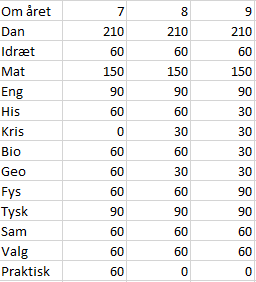
\includegraphics[scale = 0.9]{partials/graphics/antalaftimerpaaetaar.png}
  \caption{Oversigt over timetallet på et år\cite{timetal2016}.}
  \label{fig:Timetal et år}
\end{figure}


Ugeligt vil det passe med følgende:
\begin{figure}[h]
  \centering
  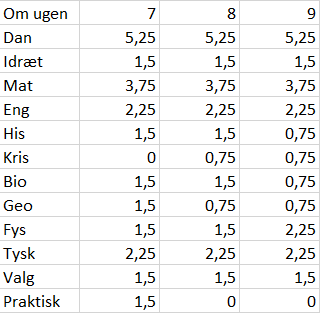
\includegraphics[scale = 0.9]{partials/graphics/antalaftimerpaaenuge.png}
  \caption{Oversigt over timetallet på en uge\cite{timetal2016}.}
  \label{fig:timetal en uge}
\end{figure}

Derudover skal programmet opfylde de specifikke krav der bliver stillet af Sofiendahlskolen. Disse krav er at alle de tunge fag, som matematik, dansk og fysik/kemi, skal lægge over middag, da eleverne ofte er trætte og ukoncentrerede efter middagspausen. Derudover skal lærernes forberedelsestimer lægge således at de har mere end en forberedelsestime ad gangen, da lærerne ikke kan nå at forberede sig til de kommende lektioner på kun en time. Derudover vil lærerne på Sofiendahlskolen gerne have mulighed for at lave samarbejde på tværs af parallel klasser, så nogle fag skal lægge på samme tidspukt på tværs af parallel klasserne\cite{interview}.